\section{自旋的发现}

\begin{quotation}
“我们已经对自旋有了最终的描述了吗?我不这样认为。” \qquad 杨振宁
\end{quotation}

我们可以通过讨论斯特恩-盖拉赫实验直接引入量子力学,而且这种引入量子力学的方式是最没有“历史包袱”的。因为斯特恩-盖拉赫实验的解释需要假设电子具有自旋1/2,自旋不同于位置(r)和动量(p),也不同于轨道角动量(L),自旋是一种没有经典对应的物理量,它是纯粹的量子对象。

\subsection{斯特恩和盖拉赫}

斯特恩\index{Otto Stern:斯特恩}(Otto Stern)是学物理化学出身,犹太人,后来追随爱因斯坦学习理论物理,但其真正擅长的还是实验物理,斯特恩是最早发展分子束技术的科学家,他用这个方法直观地验证了气体分子确实是遵从麦克斯韦分布律的,并使用这个方法测定了银原子的磁矩,甚至是质子的磁矩等等。

1922年,他与盖拉赫\index{Walter Gerlach:盖拉赫}(Walter Gerlach)合作,完成了斯特恩-盖拉赫实验。斯特恩做这个实验的初始动机是要验证玻尔提出的空间量子化\index{Space quantization: 空间量子化}(Space quantization)概念,即原子的磁矩只能取向于空间的分立方向上。当时人们认为原子磁矩来源于原子内部电子的轨道运动,电子延圆形或椭圆轨道围绕原子核运动就像环形电流一样会产生磁矩。空间量子化意味着这些圆形或椭圆轨道只能存在于特定空间取向的平面上。

但实际上斯特恩-盖拉赫实验\index{Stern-Gerlach experiment:斯特恩盖-拉赫实验}却揭示出电子本身就具有磁矩,如果我们称因轨道运动所导致的磁矩是轨道磁矩的话,这种新磁矩就称之为自旋磁矩,轨道磁矩对应轨道角动量,而自旋磁矩则对应自旋角动量。此前人们已经知道轨道角动量量子数是取整数的,而斯特恩-盖拉赫实验却显示自旋角动量量子数是半整数($1/2$)。这可以说是使物理学家大开眼界了,而且也完全超出实验的设计者斯特恩和盖拉赫的预想。

由于该实验在物理学史中的关键作用,斯特恩被授予1943年的诺贝尔物理奖(此前的1940,41,42正值二战最凶险的时刻,连续三年无人获奖,因斯特恩的犹太人身份,当时斯特恩已经逃到美国,并加入美国籍),而斯特恩本人则是被提名诺贝尔物理学奖次数最多的一位科学家,从1925-1943年他共获得了81次提名\footnote{Physicsworld.com, Nobel population 1901-50: anatomy of a scientific elite. \url{http://physicsworld.com/cws/article/print/2001/nov/05/nobel-population-1901-to-50-anatomy-of-a-scientific-elite}}。

有趣的是盖拉赫作为实验的关键合作者却未同时得奖,实际上盖拉赫在同时期也获得了30次提名,超过革末(Germer)、郎之万(Langevin)、外斯(Weiss)、梅特纳(Meitner)等同样未获得诺贝尔奖的著名物理学家的提名次数。但因德国“异议人士”卡尔·冯·奥西茨基1935年获得诺贝尔和平奖\footnote{当时奥西茨基正在服刑,纳粹德国不同意释放他去领奖,因此奥西茨基成为第一位在监狱里获得诺贝尔奖的人。\url{http://en.wikipedia.org/wiki/Carl_von_Ossietzky}},希特勒视之为对自己的羞辱,于1937年颁布法令禁止任何德国人领取任何诺贝尔奖,这使得正与纳粹合作的纯种日耳曼人盖拉赫很难有获奖的可能性。

\subsection{非均匀磁场}

实验的关键是“非均匀磁场”,斯特恩和盖拉赫制造了专门的具有特殊形状的磁铁,使得磁场基本就在$z$方向上,并且延$z$方向上是非均匀的:

\begin{eqnarray}
\vec B & =  & B_z \hat z \\
\frac{\partial }{\partial z} B_z & \neq & 0
\end{eqnarray}

我们把一个磁矩$\mu$放到磁场里,其能量是:

\begin{equation}
E(z) = - \mu \cdot B = - \mu_z B_z  
\end{equation}

磁矩\index{Magnetic moment: 磁矩}在非均匀磁场里会受到一个$z$方向上的力:

\begin{equation}
F_z = - \frac{\partial E(z)}{\partial z} = \mu_z \frac{\partial B_z}{\partial z}
\end{equation}

$\mu_z$就是磁矩在$z$方向上的分量,实验采用的粒子是银原子\index{Silver atom:银原子},即把处于高温的银原子引出来,通过准直装置飞进非均匀磁场里。

\begin{figure}[htbp]
\begin{center}
\includegraphics[width=10cm]{SGExperiment/SGexperiment.png}
\caption{斯特恩-盖拉赫实验装置示意}
%\label{default}
\end{center}
\end{figure}

银原子的原子序数是47,其电子结构可表示为:$[Kr] 4 d^{10} 5s$。

现在考虑银原子的磁矩,首先原子核的磁矩远小于电子的磁矩,这意味着我们只需要考虑银原子中电子磁矩的贡献,其次以我们今天的知识原子中满壳层或满亚壳层电子磁矩的贡献正好互相抵消(轨道磁矩和自旋磁矩都会抵消),这样我们就可判定银原子的磁矩主要来自$5s$电子的贡献。

对$s$轨道而言,轨道角动量为0,这样电子的轨道磁矩也没有了,唯一有贡献的就是$5s$电子的自旋磁矩,换句话说银原子就其磁学性质而言,它就是一个自旋$1/2$的小磁针(银原子束将分裂为上、下两束),只不过它比较重,远重于单电子的质量。

根据银原子束分裂的大小,我们可以把银原子的磁矩表示为:

\begin{equation}
\mu_z = - \frac{e}{2m } s_z
\end{equation}

这里$m$表示电子的质量,而$s_z = \pm \frac{1}{2} \hbar$,即银原子磁矩的取值有两种可能性,一正一负,或说延$z$方向一上一下,相应地银原子在非均匀磁场里的受力也是两种,延$z$方向的一上一下。这就解释了银原子在非均匀磁场里的分裂。

\begin{figure}[htbp]
\begin{center}
\includegraphics[width=10cm]{SGExperiment/sg-result.jpg}
\caption{斯特恩-盖拉赫实验的原始结果}
%\label{default}
\end{center}
\end{figure}

\subsection{连续的斯特恩-盖拉赫实验}

对我们的物理世界,选哪个方向是$z$方向是任意的,可以设想同样的实验对$x$或$y$取向的非均匀磁场也同样成立,即对$x$方向的非均匀磁场,我们会发现银原子会分裂为$x$正向和负向相同比例的两束,对应的就是自旋角动量在$x$方向上取$s_x = \pm \frac{1}{2} \hbar$的两类银原子。

真正有意思的是连续的斯特恩盖-拉赫实验\index{Stern-Gerlach experiment:斯特恩盖-拉赫实验},比如:我们可以让一束银原子通过$z$方向非均匀的磁场(记作SGz),得到在$z$方向分裂的两束,比如我们遮挡上其中一束,比如$s_z = - \frac{1}{2} \hbar$($s_z -$),我们让$s_z = \frac{1}{2} \hbar$的那一束($s_z +$)再次通过SGz装置,我们会发现从第二个SGz中出射的就只有$s_z +$的部分了。

这说明$s_z = \pm \frac{1}{2} \hbar$是互相排斥的两类,其分类标准由SGz装置定义,同时在此分类标准下分为两类又是个完全的分类(因为银原子只分裂为两束)。

我们可以让$s_z +$的成分继续通过一个$x$方向的非均匀磁场(SGx装置),此时发现银原子仍会分裂为延$x$方向正、负各50\%的两束。

这个结果是容易被人们接受的,这就相当于我们用不同于SGz所定义的分类标准对$s_z +$的成分进行第二轮筛选,其结果是分为$s_x = \pm \frac{1}{2} \hbar$($s_x \pm$)两类。

我们可以把$s_x -$的成分遮挡住,只引出$s_x +$的成分,使之再次通过$z$方向的非均匀磁场(SGz),现在的问题是银原子是会分裂为$s_z \pm$两束,还是只有$s_z +$一束?

\begin{figure}[htbp]
\begin{center}
\includegraphics[width=10cm]{SGExperiment/SequentialSGE.jpg}
\caption{连续的斯特恩-盖拉赫实验}
%\label{default}
\end{center}
\end{figure}

直觉上我们会觉得只会得到$s_z +$一束,但实验结果却是仍然分裂为$s_z \pm$两束。这里我们选择充分相信实验的结果,不去质疑实验的设计与细节,在此前提下我们应如何理解这个结果呢?

从分类的角度,这里涉及两个不同分类标准,一个是$SGz$,一个是$SGx$,第一次筛选,我们只筛选出$s_z +$的成分,然后我们继续分类,换之以$SGx$标准,得到$s_x \pm$两类,但问题是在我们进行第二次分类的时候,银原子是否能够继续保持$s_z +$这一状态呢?

在量子力学中,我们会说由于算符$s_z$和$s_x$是不对易的,因此不存在$s_z$和$s_x$同时取确定值的量子态(自旋量子数$s=0$的情形除外)。即如果我们知道银原子处在比如$s_x +$的状态,它就不可能同时处于$s_z +$的状态了。这说明理解斯特恩-盖拉赫实验对理解量子力学很重要。

理解新事情总是通过将其比拟为另一个(更熟悉的)事情来达成。比如连续的斯特恩-盖拉赫实验之所以难理解,是因为我们会把$s_z$和$s_x$想象为一个向量的在不同方向上的投影,这样$s_z$和$s_x$同时取确定值就是好理解的,而无法同时取确定值就是无法理解的。

\subsection{光学类比}

通过光学类比我们可以获得这种理解。

光波是电磁波,电磁波是横波,电场分量$\vec E$和磁场分量$\vec B$振荡的方向与电磁波传播的方向$\vec k$垂直。这样对电磁波而言就有了偏振\index{Polarized light:偏振光}的概念。

求解电磁波方程,会得到这样的关系\footnote{Electromagnetic radiation, \url{http://en.wikipedia.org/wiki/Electromagnetic_radiation};D. J. Griffiths, Introduction to Electrodynamics, pp379.},

\begin{equation}
\vec B = \frac{1}{c} \vec k \times \vec E 
\end{equation}

这里$c$是真空中得光速,这意味着对电磁波而言,我们只需考虑电场分量$\vec E$就够了。

x-偏振光:

\begin{equation}
\vec E_x = E_0 \hat x \cos (k z - \omega t )
\end{equation}

y-偏振光:

\begin{equation}
\vec E_y = E_0 \hat y \cos (k z - \omega t )
\end{equation}

偏振片能吸收特定方向振荡的电磁波,比如x-偏振片能吸收所有垂直于$x$方向的电场的能量,而让平行于$x$方向的电场的振荡穿透过去。我们可以通过旋转偏振片的方向使透射的光具有特定的偏振方向。

比如我们可以让x-偏振片逆时针旋转$45^o$得到x'-偏振光,继续旋转$90^o$得到y'-偏振光。

\begin{eqnarray}
\vec E_{x'} & = & \frac{E_0}{\sqrt 2} (\hat x + \hat y)  \cos (k z - \omega t ) \\
\vec E_{y'} & = & \frac{E_0}{\sqrt 2} ( - \hat x + \hat y)  \cos (k z - \omega t )
\end{eqnarray}

x/y-偏振光和x'/y'偏振光是对电磁波的两种不同分类方式,它们分别都是既不遗漏也不重复的分类方式。即x-偏振光中没有丝毫y-偏振光的成分,y-偏振光中也没有丝毫的x-偏振光的成分。

我们现在可以构造一个连续的偏振片的实验来类比连续的斯特恩-盖拉赫实验:首先让一束自然光通过x-偏振片,得到x-偏振光(对应$s_z +$),然后继续通过x'-偏振片,得到x'-偏振光(对应$s_x +$),最后使之通过y-偏振片。最终会有y-偏振光(对应$s_z -$)射出吗?

答案是肯定的,并且很容易理解,对x-偏振光而言,电场振荡的方向在$x$方向上,x-偏振光穿过x'-偏振片意味着垂直于$x'$方向的光会被吸收,而平行于$x'$方向的光会穿透出来,电场强度应是$\vec E_x$向$x'$方向做投影,因子为$\frac{1}{\sqrt 2}$,由于光强正比于电场强度的平方,因此正好有50\%的光会穿透过来。

现在,穿过x'-偏振片光的电场就在$x'$方向上了,再继续穿过y-偏振片,就是向$y$方向做投影,这样会再次得到因子$\frac{1}{\sqrt 2}$,...

\begin{figure}[htbp]
\begin{center}
\includegraphics[width=8cm]{Spin/E0_projection.png}
\caption{振幅为$E_0$的x线偏振光先向x'方向投影,振幅变为$\frac{E_0}{\sqrt{2}}$,最后向y方向投影,振幅变为$\frac{E_0 }{2}$。光强正比于振幅的平方,因此光强的比为:100\% : 50\% : 25\%。}
%\label{default}
\end{center}
\end{figure}

这样我们就可以对银原子的量子态(即自旋1/2的量子态)建立起一个数学表示,我们用一个二维的列向量来表示自旋1/2的量子态,$s_z +$的态对应x-偏振光,我们把它表示为:

\begin{equation}
\left| s_z + \right\rangle = \left| + \right\rangle = \left( \begin{array}{cc} 1 \\ 0 \end{array} \right)
\end{equation}

类似地,用y-偏振光对应的二维列向量来表示$s_z -$的态:

\begin{equation}
\left| s_z - \right\rangle = \left| - \right\rangle = \left( \begin{array}{cc} 0 \\ 1 \end{array} \right)
\end{equation}

用x'-偏振光对应的二维列向量来表示$s_x +$的态:

\begin{equation}
\left| s_x + \right\rangle  = \frac{1}{\sqrt 2} \left( \begin{array}{cc} 1 \\ 1 \end{array} \right)
\end{equation}

用y'-偏振光对应的二维列向量来表示$s_x -$的态:

\begin{equation}
\left| s_x - \right\rangle  = \frac{1}{\sqrt 2} \left( \begin{array}{cc} -1 \\ 1 \end{array} \right)
\end{equation}

最后还剩两个态$s_y \pm$,我们用圆偏振光(右旋和左旋)对应的二维列向量来表示:

\begin{equation}
\left| s_y \pm \right\rangle = \frac{1}{\sqrt 2} \left( \begin{array}{cc} 1 \\ \pm i \end{array} \right)
\end{equation}

这意味着我们可用二维复系数线性向量空间中的一个向量来表示一个自旋1/2的量子态。

\subsection{电子的自旋假说}

那么斯特恩-盖拉赫实验应如何解释呢?实际上它是表明电子具有新角动量——自旋角动量$S$的实验证据。自旋(spin)这个名称来自与经典图像的类别,但这个对比又是不成立的!换句话说这个名字取错了,但名字无非是个指称,物理学家似乎不太在乎这个名字会给门外汉带来误导,他们只是强调自旋是电子(或粒子)的内禀性质,和空间位置($x, y, z$)无关,既然和空间位置无关,我们也就无法把自旋想象成一种在三维空间里发生的自己围绕自己的转动了。

Uhlenbeck和Goudsmit于1925年提出电子自旋假说:

\index{Spin: 自旋}

\begin{enumerate}
    \item 每个电子具有自旋角动量$S$,$\left| S \right|^2  = s\left( {s + 1} \right)\hbar ^2  = {\textstyle{3 \over 4}}\hbar ^2 $, $s = 1/2$;

自旋角动量的$z$分量取值只有两个:$S_z  = m_s \hbar  =  \pm
{\textstyle{1 \over 2}}\hbar $


    \item 每个电子都有自旋磁矩:$\mu_s  =  - \frac{e}{m_e }S =  - g_s \frac{e}{{2m_e }}S$

自旋磁矩的$z$分量取值只有两个:$\mu_{sz}  =  - g_s \frac{e}{{2m_e
}}S_z =  - g_s \frac{e}{{2m_e }}\left( { \pm {\textstyle{1 \over
2}}\hbar } \right)$

其中:$g_s  = 2$,由于$g_L  \ne g_s
$导致电子总磁矩:$\mathord{\buildrel{\lower3pt\hbox{$\scriptscriptstyle\rightharpoonup$}}
\over \mu}  =
\mathord{\buildrel{\lower3pt\hbox{$\scriptscriptstyle\rightharpoonup$}}
\over \mu} _L  +
\mathord{\buildrel{\lower3pt\hbox{$\scriptscriptstyle\rightharpoonup$}}
\over \mu} _S  =  - \left( {g_L \mu _B
\mathord{\buildrel{\lower3pt\hbox{$\scriptscriptstyle\rightharpoonup$}}
\over L}  + g_s \mu _B
\mathord{\buildrel{\lower3pt\hbox{$\scriptscriptstyle\rightharpoonup$}}
\over S} } \right)$
与总角动量$\mathord{\buildrel{\lower3pt\hbox{$\scriptscriptstyle\rightharpoonup$}}
\over J}  =
\mathord{\buildrel{\lower3pt\hbox{$\scriptscriptstyle\rightharpoonup$}}
\over L}  +
\mathord{\buildrel{\lower3pt\hbox{$\scriptscriptstyle\rightharpoonup$}}
\over S} $
不再共线。$\mathord{\buildrel{\lower3pt\hbox{$\scriptscriptstyle\rightharpoonup$}}
\over \mu} _L $
与$\mathord{\buildrel{\lower3pt\hbox{$\scriptscriptstyle\rightharpoonup$}}
\over L}
$以及$\mathord{\buildrel{\lower3pt\hbox{$\scriptscriptstyle\rightharpoonup$}}
\over \mu} _s
$与$\mathord{\buildrel{\lower3pt\hbox{$\scriptscriptstyle\rightharpoonup$}}
\over S} $
共线,并且它们都围绕总角动量$\mathord{\buildrel{\lower3pt\hbox{$\scriptscriptstyle\rightharpoonup$}}
\over J} $
进动。考虑自旋磁矩后,单电子的朗德因子\footnote{参考扬福家《原子物理学》第162页}为:$g_J
= g_L \frac{{J^2  + L^2  - S^2 }}{{2J^2 }} + g_S \frac{{J^2  + S^2 -
L^2 }}{{2J^2 }}$

\end{enumerate}

由于在原子物理中大写的$L$, $S$,
$J$常常用来表示两个电子或多个电子的``总轨道角动量'',
``总自旋角动量'', 和``总总角动量'', 所以我们现在用小写字母$l$, $s$,
$j$来表示一个电子的``轨道角动量'', ``自旋角动量'', 和``总角动量''.
朗德因子$g_j$定义为:

\begin{center}
$g_j = $ $\mu_z$(以$\mu_B$为单位)/$j_z$(以$\hbar$为单位)
\end{center}

\begin{figure}[h]
\begin{center}
  % Requires \usepackage{graphicx}
  \includegraphics[width=5cm]{Spin/lande_factor_gj.ps}\\
  \caption{考虑轨道和自旋角动量后的电子的g因子.}\label{one electron g factor}
\end{center}
\end{figure}


总角动量: $\vec j = \vec l + \vec s$,
我们在角动量矢量模型的基础上展开以下计算, 这意味着,

\begin{equation*}
|\vec j| =\hbar \sqrt{j(j+1)}; |\vec l| =\hbar \sqrt{l(l+1)}; |\vec
s| =\hbar \sqrt{s(s+1)}
\end{equation*}

$\vec s$和$\vec l$围绕总角动量$\vec j$飞快旋进, 另一方面磁矩分别为:

\begin{equation*}
\vec \mu_s = - g_s \frac{\mu_B}{\hbar}  \vec s; \vec \mu_l = - g_l
\frac{\mu_B}{\hbar}  \vec l;
\end{equation*}

总磁矩为: $\vec \mu = \vec \mu_l + \vec \mu_s$,
但现在的问题是由于$g_l \ne g_s$, $\vec \mu$和$\vec
j$不在一条直线上了, 考虑到$\vec \mu$是围绕$\vec j$快速旋进的,
所以只有$\vec \mu$向$\vec j$方向的投影$\vec \mu_j$才是有效的,
垂直于$\vec j$方向的贡献相互抵消了。因此:

\begin{equation*}
\vec \mu_j = \vec \mu_s \cos(\vec s, \vec j) + \vec \mu_l \cos(\vec
l, \vec j)
\end{equation*}

根据三角形的关系,

\begin{center}
$|\vec l|^2 = |\vec j|^2 + |\vec s|^2 -2|\vec j|\cdot|\vec
s|\cos(\vec s,\vec j)$;

$|\vec s|^2 = |\vec j|^2 + |\vec l|^2 -2|\vec j|\cdot|\vec
l|\cos(\vec l,\vec j)$.
\end{center}

这里$(\vec s, \vec j)$表示向量$\vec s$和向量$\vec j$的夹角; 类似地,
$(\vec l, \vec j)$表示向量$\vec l$和向量$\vec j$的夹角.

因此, $\cos(\vec s,\vec j) = \frac{|\vec j|^2 + |\vec s|^2 - |\vec
l|^2}{2|\vec j|\cdot|\vec s|}$, $\cos(\vec l,\vec j) = \frac{|\vec
j|^2 + |\vec l|^2 - |\vec s|^2}{2|\vec j|\cdot|\vec l|}$. 然后,
把它们代入$\vec \mu_j$的表达式中.

\begin{equation*}
\vec \mu_j = - g_s \frac{\mu_B}{\hbar} \vec s \cdot \frac{|\vec j|^2
+ |\vec s|^2 - |\vec l|^2}{2|\vec j|\cdot|\vec s|}  - g_l
\frac{\mu_B}{\hbar} \vec l \cdot \frac{|\vec j|^2 + |\vec l|^2 -
|\vec s|^2}{2|\vec j|\cdot|\vec l|}
\end{equation*}


我们把$\vec \mu_j$写作$- g_j \frac{\mu_B}{\hbar} \vec j$,
由此可得到$g_j$的表达式:

\begin{equation}\label{gj formula for one electron}
g_j = g_s \frac{|\vec j|^2 + |\vec s|^2 - |\vec l|^2}{2|\vec j|^2} +
g_l \frac{|\vec j|^2 + |\vec l|^2 - |\vec s|^2}{2|\vec j|^2}
\end{equation}

考虑到对角动量而言, 满足以下本征方程:

\begin{eqnarray*}
% \nonumber to remove numbering (before each equation)
  \hat s^2 \chi_{s,m_s}  &=& s(s+1)\hbar^2 \chi_{s,m_s}\\
  \hat l^2 \psi_{l,m_l} &=& l(l+1)\hbar^2 \psi_{l,m_l} \\
  \hat j^2 \phi_{j,m_j} &=& j(j+1)\hbar^2 \phi_{j,m_j}
\end{eqnarray*}

公式(\ref{gj formula for one electron})可改写为:

\begin{equation*}
g_j = g_s \frac{\hat j^2 + \hat s^2 - \hat l^2}{2\hat j^2} + g_l
\frac{\hat j^2 + \hat l^2 - \hat s^2}{2\hat j^2} = \frac{g_s +
g_l}{2} + \left(\frac{g_s - g_l}{2} \right)\left(\frac{\hat s^2 -
\hat l^2}{\hat j^2} \right)
\end{equation*}

对电子而言, $g_s = 2$, $g_l =1$, 上式可重新改写为:

\begin{equation}\label{gj formula for gs2 gl1}
g_j = \frac{3}{2}+\frac{1}{2}\left(\frac{\hat s^2 -\hat l^2}{\hat
j^2} \right)
\end{equation}

最后总角动量$\vec j$是围绕$z$轴飞快旋进的, $j_z = m_j \hbar, m_j =
j, j-1, ..., -j$; $\vec \mu_j$在$z$轴上的取值是:$(\vec \mu_j )_z =
-g_j \mu_B m_j$.

\textbf{练习}:考虑电子$s=1/2$, $l=1$,
$j$可以是$3/2$和$1/2$(根据角动量的矢量模型, $j = l+s, l+s-1,...,
|l-s|$), 分别求$g_j$.

解: 对$s=1/2$, $l=1$, $j=3/2$,
这样的态在原子物理中一般记作${}^2P_{3/2}$, $g_j = 4/3$;
对$j=1/2$(${}^2P_{1/2}$), $g_j = 2/3$.

值得注意的是, 公式(\ref{gj formula for gs2
gl1})虽然是针对``单电子''推出的,
但即使对``对原子的总角动量(也就是对原子的总磁矩)有贡献的电子数目不止一个'',
这个公式在大多数情况下仍然适用。即只要把$s, l, j$换成$S, L, J$即可,
公式(\ref{gj formula for gs2 gl1})变为:


\begin{equation*}
g_J = \frac{3}{2}+\frac{1}{2}\left(\frac{\hat S^2 -\hat L^2}{\hat
J^2} \right)
\end{equation*}

这个公式成立的前提是RS耦合(Russoll-Saundors,
又称L-S耦合)占优势的情况,
即所有的电子先分别耦合(``矢量''相加)成总自旋(S)和总轨道角动量(L),
然后再耦合成总角动量J. 即:

\begin{equation*}
\left(s_1,s_2,...  \right)\left(l_1,l_2,l_3,...
\right)=\left(L,S\right)=J
\end{equation*}


我们引入原子态记号: ${}^{2S+1}L_J$来标记原子的不同态,
其中:$2S+1$是自旋多重度,
  $L$表示轨道角动量, $J$是总角动量;

对轨道角动量,我们经常用字母$S, P, D, F, G, ...$来表示$L =
0,1,2,...$。具体见下表:


\begin{center}
\begin{tabular}{|c|c|c|c|c|c|c|c|c|c|}
  \hline
  % after \\: \hline or \cline{col1-col2} \cline{col3-col4} ...
  0 & 1 & 2 & 3 & 4 & 5 & 6 & 7 & 8 & ... \\
  \hline
  S & P & D & F & G & H & I & K & L & ... \\
  \hline
\end{tabular}
\end{center}



\subsection{自旋的物理图像}

电子自旋是电子内禀自由度,是量子力学中全新的物理量,并没有经典的对应物。(如轨道角动量在经典物理学中对应为$\mathord{\buildrel{\lower3pt\hbox{$\scriptscriptstyle\rightharpoonup$}}
\over r}  \times
\mathord{\buildrel{\lower3pt\hbox{$\scriptscriptstyle\rightharpoonup$}}
\over p} $)


Uhlenbeck和Goudsmit最初把电子自旋理解为电子的自转,但这样做会面临很多困难:

\begin{enumerate}

\item 迄今为止的实验, 未发现电子有尺寸的下限, 如果电子的尺寸为0, 如何建立电子自转的图像?

    \item 假设电子是有限大小的球体(设为$r_e $),电荷在球体内按某种规律分布:由于旋转导致的自旋角动量$S \propto m_e r_e ^2 \omega  \sim \frac{\hbar }{2}$

根据爱因斯坦质能关系:$m_e c^2  \sim \frac{{e^2 }}{{r_e
}}$,可以估计出电子的经典半径:$r_e  \sim \frac{{e^2 }}{{m_e c^2 }}$


电子自转角速度:$\omega  \sim \frac{\hbar }{{2m_e r_e^2 }}$

电子表面运动切线速度:$v \sim \omega r_e  \sim \frac{\hbar }{{2m_e
r_e }} \sim \frac{{\hbar c^2 }}{{2e^2 }} \sim \frac{c}{{2\alpha }}
\sim 70c \gg c$,远大于光速,与相对论不符。



    \item 按照量子力学,如果假设自旋是来自于电子的转动,哈密顿算符为:$H = \frac{{L^2 }}{{2I_e }}$

其本征函数为$Y_{lm}$(定点转动),$\frac{1}{{\sqrt {2\pi }
}}e^{im\varphi }
$(定轴转动),$l$、$m$都是整数,这样将无法解释电子自旋为半奇数的实验事实\footnote{考虑波函数:$\Phi
_m (\varphi ) = \frac{1}{{\sqrt {2\pi } }}e^{im\varphi } $,$m =
\pm {\textstyle{1 \over 2}}$,将导致波函数的不连续:$\Phi
_{{\textstyle{1 \over 2}}} (0) \ne \Phi _{{\textstyle{1 \over 2}}}
(2\pi )$;如波函数是以$4 \pi$为周期,则有边界条件:$\Phi
_{{\textstyle{1 \over 2}}} (0) = \Phi _{{\textstyle{1 \over 2}}}
(4\pi )$, 即电子在空间中``转动''$4 \pi$回复到初始位置。}。

    \item 质子、中子的自旋也是$1/2$,目前自然界中发现的基本粒子自旋都是整数或半奇数倍\footnote{参考扬福家《原子物理学》第423页},
而不存在自旋为${\textstyle{1 \over 3}},{\textstyle{2 \over
3}},{\textstyle{1 \over
4}},...$这样的粒子。自旋是半整数的粒子(比如1/2, 3/2等)叫费米子,
自旋是整数的粒子(比如0, 1等)叫玻色子. 电子, 质子, 中子等是费米子,
而光子是玻色子.
   \end{enumerate}


因此自旋导致的物理现象是纯粹的量子力学效应,
讨论自旋可以最``干净''地引入量子概念, 因为自旋无经典对应,
我们也就不会受到经典图像的干扰。



\subsection*{物理常数}

\begin{itemize}
  \item 玻尔磁子: $\mu_B = \frac{e\hbar}{2m_e} = 0.9274 \times 10^{-23} J \cdot T^{-1}$
  \item 沿$z$轴磁矩: $\left( \vec \mu \right)_z = - g_j m_j \mu_B$,
  $m_j = j, j-1, ..., -j$
  \item 朗德因子: $g_S = 2$, $g_L =1$, $g_J =  \frac{g_S +
g_L}{2} + \left(\frac{g_S - g_L}{2} \right)\left(\frac{\hat S^2 -
\hat L^2}{\hat J^2} \right) $
  \item 磁矩在磁场中的势能: $U_m = -\vec \mu \cdot \vec B $
\end{itemize}


~~

\subsection*{练习}

\begin{enumerate}
\item 

斯特恩-盖拉赫实验,银原子束从温度为600K的炉子跑出来,经过准直装置后,通过一个0.1米长的非均匀磁场,磁场的梯度是$\frac{\partial B_z}{\partial z} = 10^3$特斯拉/米。银原子从非均匀磁场跑出来后又继续“飞”了1米,求最终银原子在靶上的分裂宽度是多少。(假设银原子的平均速度为$v$,它的平均动能是$\frac{M v^2}{2} = \frac{3 k_B T}{2}$,这里$M$是银原子的质量,$k_B$是玻尔兹曼因子。)

\item
  试证:原子在${}^6G_{3/2}$状态的磁矩等于0,并根据矢量模型对这一事实作出解释。

解:对态:${}^6G_{3/2}$, $S=\frac{5}{2}$, $L=4$, $J=\frac{3}{2}$,
J的可能取值是$\frac{13}{2}$, $\frac{11}{2}$, $\frac{9}{2}$,
$\frac{7}{2}$, $\frac{5}{2}$, $\frac{3}{2}$,
$J=\frac{3}{2}$意味着$\vec L$和$\vec S$正好``最大程度''地相互抵消,
即: $J = |L-S|=\frac{3}{2}$.

把$S=\frac{5}{2}$, $L=4$, $J=\frac{3}{2}$代入$g_J =  \frac{g_S +
g_L}{2} + \left(\frac{g_S - g_L}{2} \right)\left(\frac{\hat S^2 -
\hat L^2}{\hat J^2} \right) $计算可得:$g_J =0$, 注意这里: $\hat S^2
= S(S+1)\hbar^2 = \frac{35}{4}\hbar^2$, $\hat L^2 =
L(L+1)\hbar^2=20\hbar^2$, $\hat J^2 =
J(J+1)\hbar^2=\frac{15}{4}\hbar^2$.

如果要用矢量模型理解$g_J =0$, 我们首先需要构造$\vec J$, $\vec S$,
$\vec L$组成的三角形, 即构造边长分别为:


$|\vec J|=\hbar \sqrt{J(J+1)}=\frac{\sqrt {15}}{2}\hbar=1.936\hbar$,


$|\vec S|=\hbar\sqrt{S(S+1)}=\frac{\sqrt{35}}{2}\hbar=2.958\hbar$,


和$|\vec L|=\hbar\sqrt{L(L+1)}=\sqrt {20} \hbar=4.472\hbar$

的三角形. 作图可证明: $\vec \mu = \vec \mu_S + \vec \mu_L$
垂直于$\vec J$, 而$\vec \mu$是要向$\vec J$做投影的, 得到$\vec
\mu_J=0$, 因此态:${}^6G_{3/2}$, $S=\frac{5}{2}$的磁矩为0.


  \item 只考虑盐酸分子(HCl)的转动能, 即$H = L^2/2I$, 这里$L$是轨道角动量,
$I$是转动惯量, 估算盐酸分子的转动能级,
基态和第一激发态间能量差(用eV表示)是多少?
对应光波波长(用nm表示)是多少?

\end{enumerate}

\subsection*{阅读与思考}

阅读维尔泽克(Frank Wilczek, 1951-,
2004年诺贝尔物理奖得主)的文章``从电子学到任意子学''(From electronics
to anyonics); 英文:
\url{http://www.frankwilczek.com/Wilczek_Easy_Pieces/394_From_Electronics_to_Anyonics.pdf}.